\documentclass[11pt]{article}
\usepackage[a4paper,margin=2.2cm]{geometry}
\usepackage[T1]{fontenc}
\usepackage{lmodern}
\usepackage{microtype}
\usepackage{amsmath}
\usepackage{booktabs}
\usepackage{graphicx}
\usepackage[numbers]{natbib}
\usepackage[hidelinks]{hyperref}
\usepackage{xcolor}
\usepackage{xurl}
\usepackage[section]{placeins}
\usepackage{caption}
\captionsetup{skip=6pt}
% Generated tables use table* for a two-column paper; in this one-column report they float like table
\makeatletter
\renewenvironment{table*}[1][]{\@float{table}[!htbp]}{\end@float}
\makeatother

% Tables and figures are generated by notebooks/99_final_eval.ipynb; never edit them by hand
\graphicspath{{../../results/final_eval/figures/}}
\newcommand{\tbl}[1]{\input{../../results/final_eval/paper/#1.tex}}
\newcommand{\todo}[1]{\textcolor{red}{[TODO: #1]}}

\title{Zero-shot prompted LLM baselines for sexism detection\\[2pt]
\large CMSB, EDOS and EXIST 2025 (English): test-set results}
\author{Pawan Sapkota Sharma}
\date{20 October 2026 \\ \small evaluation run \texttt{20261020\_all\_all\_llms\_finaleval\_s42}}

\begin{document}
\maketitle

\begin{abstract}
We report test-set results for 15 open-weight instruct language models ($\leq$8B parameters) used as zero-shot classifiers on seven sexism-detection tasks:
\begin{itemize}
  \item CMSB binary;
  \item EDOS Tasks A, B and C;
  \item EXIST 2025 Tasks 1.1, 1.2 and 1.3 (English tweets).
\end{itemize}
Every label is scored from the next-token probability of the answer tokens: Yes/No, or an option letter. No free-text generation is used.

A label whose answer tokens receive less than half of the next-token probability mass is treated as a soft refusal and scored as wrong. This rule, the decision thresholds and all statistical tests were fixed before any test label was read.

Results:
\begin{itemize}
  \item \textbf{Best macro-F1 per task:} CMSB 0.821 (Granite~4.1-8B), EDOS~A 0.712 (Gemma-4~E4B), EDOS~B 0.508 (Falcon-H1-7B), EDOS~C 0.256 (Gemma-4~E4B).
  \item \textbf{Refusals} are absent on Yes/No tasks. They are frequent on the 11-way EDOS~C task for three models (83--99\% of posts).
  \item \textbf{Bias:} most models over-predict the sexist class.
  \item \textbf{Agreement} between models falls sharply from binary to fine-grained tasks.
\end{itemize}
Overall, small open models detect sexism reasonably well without any training data at the binary level, but fine-grained categorisation remains far from solved. How non-answers are scored materially changes fine-grained results. EXIST scores are pending official evaluation.
\end{abstract}

\section{Motivation and scope}
Detecting sexism in online posts, and especially telling apart its forms (threats, derogation, stereotyping, and so on), normally needs large amounts of expert-annotated training data, which is expensive to produce. Small open-weight instruct models offer an alternative. They can be run locally, at low cost and without sending data to a third party, and asked to label posts directly from a written definition, with no training at all.

This study asks three questions:
\begin{itemize}
  \item How far does this zero-shot approach go, from binary detection to 11-way categorisation, across three established benchmarks?
  \item Where does it fail?
  \item How should such models be scored fairly when they do not answer in the required format?
\end{itemize}
The results also serve as a reference point for supervised systems evaluated on the same splits.

Every number below comes from the evaluation run named on the title page. Its tables and figures are generated by \texttt{notebooks/99\_final\_eval.ipynb} from the 105 test runs of batch \texttt{20261020\_all\_all\_llms\_batch\_s42}.

All results are for a single seed (42) and a single prompt per task. Differences between models therefore describe this setting. They are not general claims about the models.

\section{Data and tasks}\label{sec:data}
Models are scored against \emph{gold labels}: the reference answers assigned to each post by the datasets' human annotators. EXIST provides two forms of gold label:
\begin{itemize}
  \item \emph{hard}: one answer per tweet, by majority vote of its six annotators;
  \item \emph{soft}: the share of annotators choosing each answer, e.g.\ 83\% YES and 17\% NO, which preserves annotator disagreement.
\end{itemize}

Each dataset is evaluated on its own official test split and task definitions (Table~\ref{tab:tasks}). All models receive the same normalised text. Normalisation unescapes HTML, applies Unicode NFC, replaces user mentions with \texttt{[USER]} and URLs with \texttt{[URL]}, and collapses whitespace; there is no lowercasing.

\begin{table}[t]
\centering\small
\caption{Test sets and scoring subsets.}\label{tab:tasks}
\begin{tabular}{llllr}
\toprule
Dataset & Task & Type & Classes & Test $n$ (scored) \\
\midrule
CMSB \citep{samory2021callme} & binary & binary & sexist / not & 1{,}126 \\
EDOS \citep{kirk2023semeval} & A & binary & sexist / not & 4{,}000 \\
 & B & single-label & 4 categories & 4{,}000 (970) \\
 & C & single-label & 11 vectors & 4{,}000 (970) \\
EXIST 2025, en \citep{plaza2025exist} & 1.1 & binary & YES / NO & 978 (EvALL) \\
 & 1.2 & single-label & 4 intentions (incl.\ NO) & 978 (EvALL) \\
 & 1.3 & multi-label & 5 categories & 978 (EvALL) \\
\bottomrule
\end{tabular}
\end{table}

\paragraph{CMSB.} We use the annotated subset only, excluding the unannotated posts of the \texttt{other} source. All of those posts are non-sexist, so including them would add a source shortcut. The test split has 1{,}126 posts, 361 of them sexist.

The CMSB split is a fixed 70/10/20 split, grouped so that originals, their adversarial modifications and duplicate texts share a split. After normalisation, 33 test posts have the same text as a train or dev post. We report results with and without them.

\paragraph{EDOS.} Official test split: 4{,}000 posts, 970 of them sexist. Models were run on all 4{,}000 posts for Tasks B and C. B and C are scored on the 970 gold-sexist posts, i.e.\ given the gold sexist/not-sexist decision rather than end to end.

Gold class counts:
\begin{itemize}
  \item \textbf{B:} derogation 454, animosity 333, prejudiced discussions 94, threats 89.
  \item \textbf{C:} the 11 vectors range from 205 posts (2.1, descriptive attacks) to 14 (3.4, condescending explanations).
\end{itemize}

\paragraph{EXIST 2025.} We use the English test tweets (978); Spanish is out of scope for now. The organisers released the test tweets without their gold labels, as is usual in shared tasks, so that systems cannot be tuned on the test answers. Test scores are obtained by submitting predictions to the official evaluation service (Section~\ref{sec:exist}). Until then, EXIST appears here only in analyses that need no labels.

\section{Models and prompting}\label{sec:models}
\paragraph{Models.} The pool has 15 open-weight instruct models, each $\leq$8B total parameters by its model-card figure (Appendix Table~\ref{tab:models}). All are pinned to a fixed Hugging Face revision and run with stock \texttt{transformers}~5.20.1 and PyTorch~2.11.0 on one NVIDIA A100-SXM4-80GB.
\begin{itemize}
  \item Thinking/reasoning modes are disabled.
  \item Ministral-3-3B ships FP8 weights only. It is dequantised to bf16, since the A100 has no native FP8.
  \item Inference uses batch size~1.
\end{itemize}

\paragraph{Prompts.} Each prompt has a fixed system message (``You are an expert annotator who labels social media posts for sexism.''; ``tweets'' for EXIST) and a user turn with the post. Label definitions come from each dataset's own taxonomy:
\begin{itemize}
  \item CMSB: the content/phrasing definition of \citet{samory2021callme};
  \item EDOS: the category and vector definitions of \citet{kirk2023semeval};
  \item EXIST: the task guidelines.
\end{itemize}
Prompt templates are versioned YAML files, and their SHA-256 is stored with every prediction. One template version was used per task.

\paragraph{Log-probability scoring.} Binary and multi-label tasks ask one question per label (``Is this post \emph{sexist} according to the definition? Answer with Yes or No only.''). We read the next-token distribution at the first reply position of the chat template, with no prefilled reply. We then compute
\begin{itemize}
  \item $P(\text{Yes})$: summed over the single-token variants \emph{Yes, \textvisiblespace Yes, yes, \textvisiblespace yes, YES};
  \item $P(\text{No})$: summed the same way;
  \item the answer mass $m = P(\text{Yes}) + P(\text{No})$.
\end{itemize}
A label is predicted positive when $P(\text{Yes})/m \geq 0.5$.

Single-label tasks (EDOS B/C, EXIST 1.2) list the classes as lettered options. The prediction is the arg-max of the per-letter probabilities (each letter with and without a leading space), and $m$ is their sum. The softmax is computed in float32. No exact 0.5 scores occur on the test runs.

\section{Evaluation protocol}\label{sec:protocol}
The protocol was recorded in the experiment log on 20 October 2026, before the evaluation notebook read any test label. No dev runs were made. All thresholds are therefore fixed a priori rather than tuned (Section~\ref{sec:limits}).

\paragraph{Soft refusals.} A label is a soft refusal when $m < 0.5$, i.e.\ the model puts most of its next-token probability on tokens that are not a valid answer. Refusals are recorded per (post, label).

Under \emph{strict} scoring a refused label counts as wrong:
\begin{itemize}
  \item binary: the opposite of the gold label;
  \item single-label: a ``refused'' prediction that belongs to no class.
\end{itemize}
A refusal is never mapped to a class. A sensitivity analysis over cutoffs $\{\text{none}, 0.1, 0.5, 0.9\}$ was declared in advance; it is reported, never used to choose.

\paragraph{Fair subset.} The posts on which all 15 models answered every label. It allows a head-to-head comparison free of refusal effects.

\paragraph{Metrics.} The primary metric is macro-F1 over classes, chosen because of class imbalance. We also report accuracy and the F1 of the sexist class for binary tasks.

\paragraph{Uncertainty and tests.} For each model we give 95\% percentile bootstrap CIs over posts \citep{efron1993bootstrap}, with $B=10{,}000$ resamples and seed~42. All models share the same resample indices.

Each model is compared with the best model of its task:
\begin{itemize}
  \item binary tasks: an exact McNemar test \citep{mcnemar1947};
  \item EDOS B/C: a paired bootstrap of the macro-F1 difference \citep{bergkirkpatrick2012significance}.
\end{itemize}
The $p$-values get Holm correction over the 14 comparisons per task \citep{holm1979}, with $\alpha = 0.05$.

Agreement between models is Fleiss' $\kappa$ \citep{fleiss1971}. Calibration is the expected calibration error (ECE) with 10 equal-width bins \citep{guo2017calibration}.

\section{Results}\label{sec:results}

\subsection{Main results}
\tbl{main}

\begin{figure}[t]
\centering
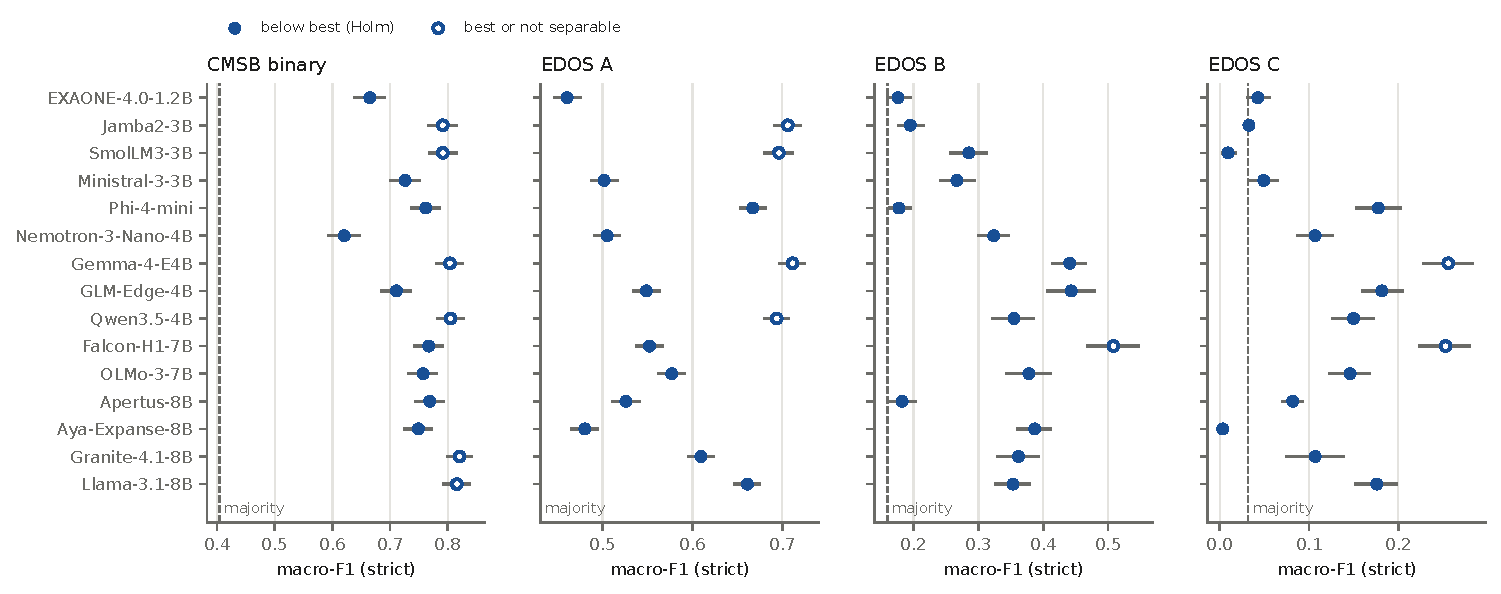
\includegraphics[width=\textwidth]{main_macro_f1_ci.pdf}
\caption{Test macro-F1 with 95\% bootstrap CIs (strict scoring, cutoff 0.5). Models are sorted by size. Hollow markers: best model, or not significantly different from it after Holm correction. Dashed line: majority-class baseline.}
\label{fig:main}
\end{figure}

Table~\ref{tab:main} and Figure~\ref{fig:main} give strict test macro-F1.
\begin{itemize}
  \item \textbf{CMSB:} the best model is Granite~4.1-8B, 0.821 [0.797, 0.843]. Five others are not significantly different from it: Llama-3.1-8B, Qwen3.5-4B, Gemma-4~E4B, Jamba2-3B and SmolLM3-3B. All 15 models are above the majority-class baseline (0.405); the median model reaches 0.767.
  \item \textbf{EDOS~A:} Gemma-4~E4B is best, 0.712 [0.696, 0.726], with Jamba2-3B and SmolLM3-3B not separable from it. Accuracy is a poor guide here: with 24\% sexist posts the majority class reaches 0.758 accuracy, and only Gemma-4~E4B, Jamba2-3B and SmolLM3-3B exceed it (Table~\ref{tab:secondary}).
  \item \textbf{EDOS~B} (4 classes): Falcon-H1-7B is best, 0.508 [0.466, 0.549]. Every other model is significantly below it. The median is 0.353.
  \item \textbf{EDOS~C} (11 classes): Gemma-4~E4B (0.256) and Falcon-H1-7B (0.253) are best and not separable. The median is 0.107. Four models (Aya Expanse~8B, SmolLM3-3B, Jamba2-3B, EXAONE-4.0-1.2B) score 0.003--0.043, close to the majority-class reference (0.032).
\end{itemize}
No model is best on all four labelled tasks. Model rankings also differ between the binary and the fine-grained tasks: Jamba2-3B and SmolLM3-3B are among the top models on CMSB and EDOS~A, and among the bottom on EDOS~C.

\subsection{Soft refusals}
\tbl{refusal}

On every Yes/No task, no label of any model falls below the 0.5 mass cutoff (Table~\ref{tab:refusal}). This covers CMSB, EDOS~A, EXIST 1.1 and the five EXIST 1.3 labels.

Refusals concentrate in the lettered-option tasks:
\begin{itemize}
  \item \textbf{EDOS~C:} Aya Expanse~8B 98.6\% of posts, SmolLM3-3B 98.3\%, Granite~4.1-8B 83.0\%, Gemma-4~E4B 13.5\%, Ministral-3-3B 9.8\%.
  \item \textbf{EXIST 1.2:} Granite 16.8\%.
\end{itemize}
For Aya on EDOS~C, the most probable next token is ``The'' or ``Based'' on 3{,}940 of the 4{,}000 posts, rather than an option letter. The model starts a free-text answer instead of choosing a letter.

As a consequence, the fair subset is empty for EDOS~C: no post was answered by all 15 models. For EDOS~B it keeps 865 of 970 posts, and fair-subset scores stay within 0.023 of the strict scores (Table~\ref{tab:secondary}).

\subsection{Sensitivity to the refusal cutoff}
\tbl{sensitivity}

Between no cutoff and the primary 0.5 cutoff, no CMSB or EDOS~A score changes. On EDOS~B/C the cutoff matters for the models that refuse (Table~\ref{tab:sensitivity}):
\begin{itemize}
  \item EDOS~C: Aya Expanse falls from 0.116 to 0.003, SmolLM3 from 0.109 to 0.009, Granite from 0.171 to 0.107.
  \item EDOS~B: SmolLM3 falls from 0.312 to 0.285.
\end{itemize}
These models' fine-grained scores depend on how refusals are treated, so both numbers should be reported for them. At 0.9, SmolLM3, Ministral-3 and Apertus fall to 0 on both tasks, and Aya and Granite drop sharply on EDOS~C. Most other models are unchanged.

\subsection{Secondary metrics and leaked posts}
\tbl{secondary}

Removing the 33 CMSB test posts whose normalised text also occurs in train/dev changes macro-F1 by at most 0.002 for any model (Table~\ref{tab:secondary}). The CMSB comparison is therefore not driven by these posts.

\subsection{Error analysis}
\begin{figure}[t]
\centering
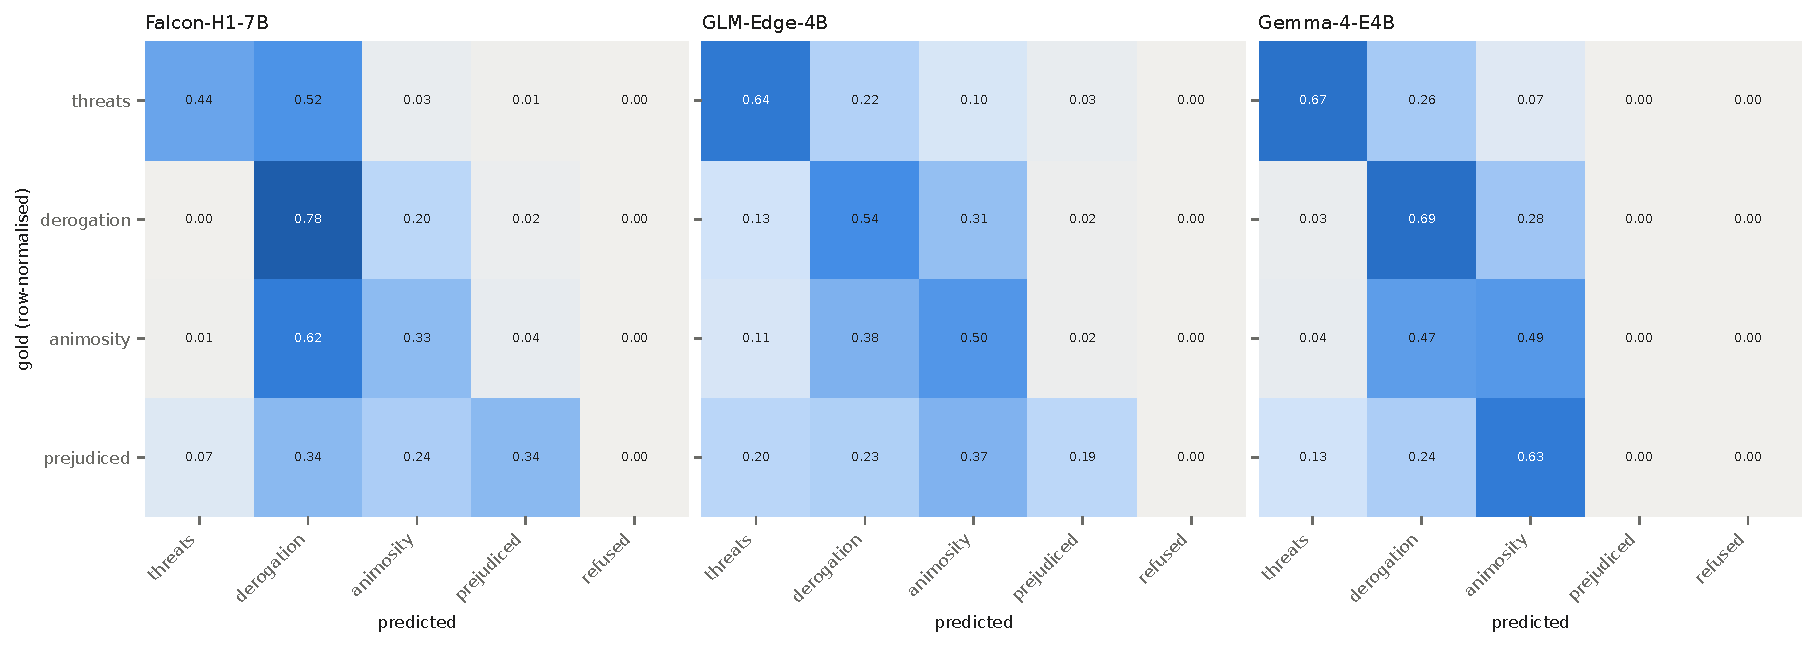
\includegraphics[width=\textwidth]{confusion_top3_task_b.pdf}
\caption{EDOS~B: row-normalised confusion matrices of the three best models on the 970 gold-sexist test posts.}
\label{fig:confb}
\end{figure}

\begin{figure}[t]
\centering
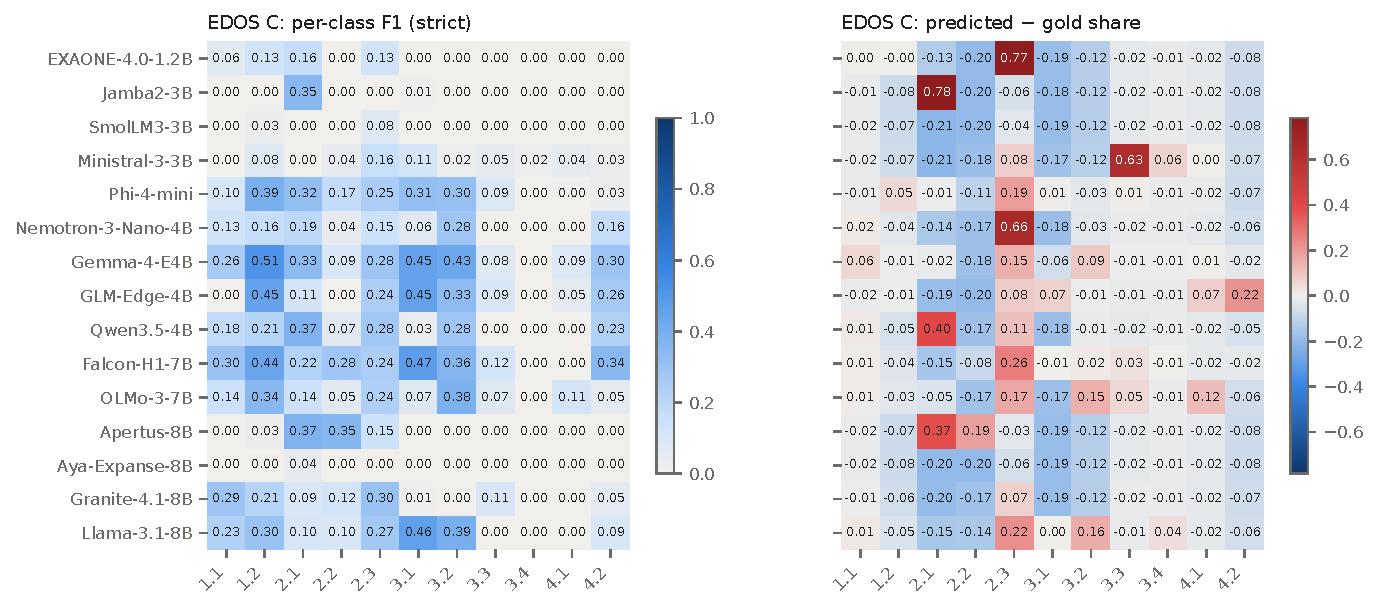
\includegraphics[width=\textwidth]{per_class_task_c.pdf}
\caption{EDOS~C: per-class F1 (left) and predicted minus gold class share (right; red = over-predicted).}
\label{fig:perc}
\end{figure}

\paragraph{EDOS~B.} The three best models confuse \emph{animosity} with \emph{derogation} (Figure~\ref{fig:confb}). Falcon-H1-7B labels 62\% of animosity posts as derogation. \emph{Prejudiced discussions} is the hardest category: Falcon-H1-7B recovers 34\% of them, GLM-Edge-4B 19\%, and Gemma-4~E4B never predicts it.

\paragraph{EDOS~C.} Several models concentrate their predictions on one vector (Figure~\ref{fig:perc}):
\begin{itemize}
  \item Jamba2-3B: 2.1 (78 points above its gold share);
  \item EXAONE-4.0-1.2B and Nemotron-3-Nano-4B: 2.3;
  \item Ministral-3-3B: 3.3.
\end{itemize}
This produces their near-baseline macro-F1. The rare vectors 3.3, 3.4 and 4.1 have F1 $\leq$ 0.12 for every model.

\subsection{Over-prediction and calibration}
\tbl{calibration}

\begin{figure}[t]
\centering
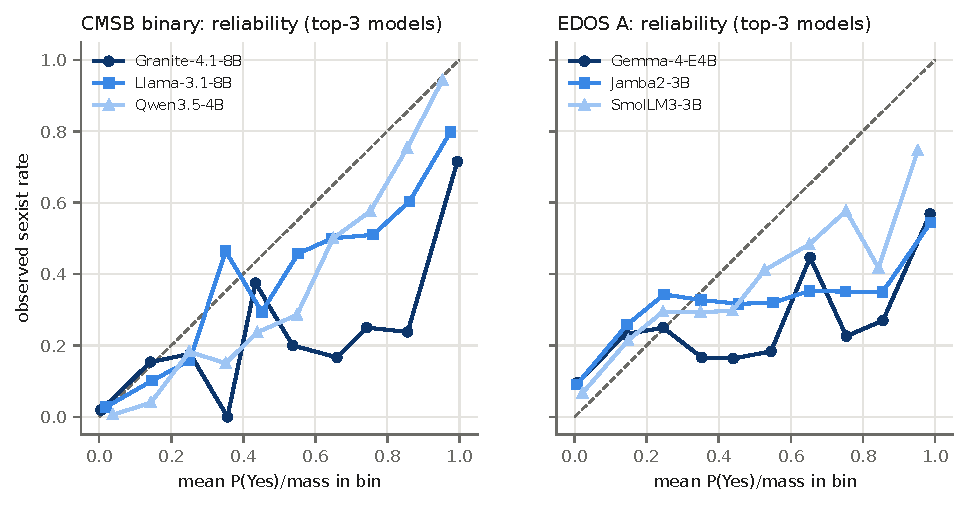
\includegraphics[width=0.8\textwidth]{calibration_top3.pdf}
\caption{Reliability diagrams of $P(\text{Yes})/m$ for the three best models per binary task (10 equal-width bins).}
\label{fig:cal}
\end{figure}

Most models label more posts as sexist than the gold rate (Table~\ref{tab:calibration}).
\begin{itemize}
  \item \textbf{CMSB} (gold 0.321): 14 of 15 models over-predict, with predicted rates up to 0.689.
  \item \textbf{EDOS~A} (gold 0.242): all 15 over-predict, with predicted rates from 0.259 to 0.760.
\end{itemize}
ECE ranges from 0.034 to 0.325 on CMSB and from 0.094 to 0.508 on EDOS~A. In the reliability diagrams (Figure~\ref{fig:cal}), even the best EDOS~A models give scores near 1 to posts of which only about 55\% are gold-sexist. The scores should therefore not be read as probabilities without recalibration.

\subsection{Agreement between models}
\tbl{agreement}

Fleiss' $\kappa$ across the 15 models (Table~\ref{tab:agreement}) is moderate on the binary tasks: 0.57 on CMSB, 0.43 on EDOS~A, 0.49 on EXIST 1.1. It is 0.44 averaged over the EXIST 1.3 labels. It is low on the single-label tasks: 0.20 on EDOS~B, 0.12 on EXIST 1.2 and 0.05 on EDOS~C. Pairwise agreement is shown in Appendix Figure~\ref{fig:pair}.

\subsection{Model size}
\begin{figure}[t]
\centering
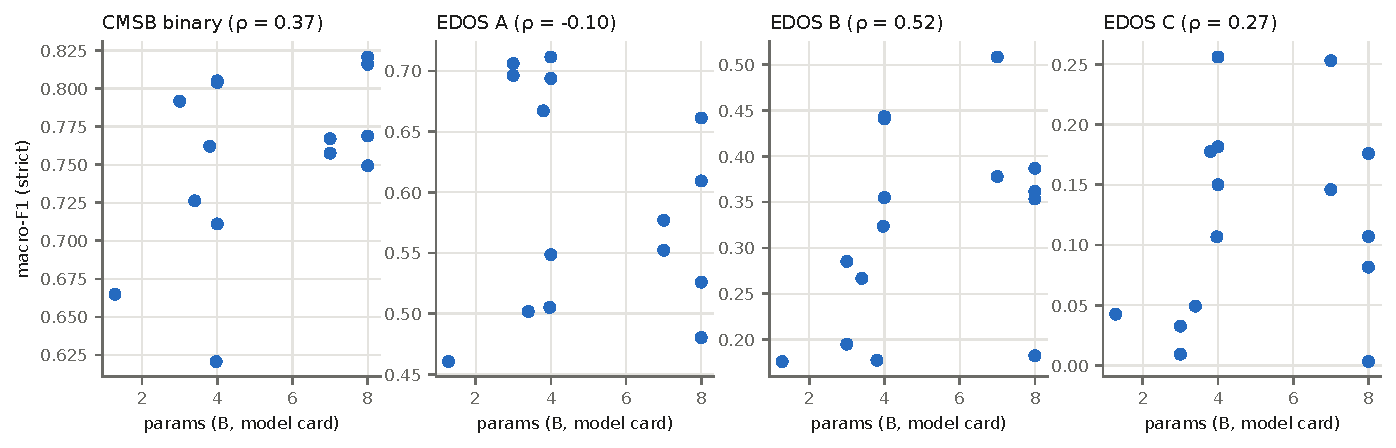
\includegraphics[width=\textwidth]{size_vs_f1.pdf}
\caption{Model-card parameter count against strict test macro-F1 (Gemma-4~E4B is plotted at 4B).}
\label{fig:size}
\end{figure}

The Spearman correlation between model-card size and macro-F1 (Figure~\ref{fig:size}) is
\begin{itemize}
  \item 0.37 on CMSB;
  \item $-0.10$ on EDOS~A;
  \item 0.52 on EDOS~B ($p=0.045$, uncorrected);
  \item 0.27 on EDOS~C.
\end{itemize}
With 15 models, one seed and a narrow size range (1.28--8B), this is descriptive only. It does not support a size trend.

\section{EXIST 2025}\label{sec:exist}
As of 20 October 2026 we found no public release of the EXIST 2025 test gold labels. They are held by the organisers' evaluation platform, EvALL (\url{https://evall.uned.es}), which scores uploaded predictions against the hidden labels. EXIST 2025 is listed in the EvALL 2.0 task repository, so predictions can still be evaluated after the campaign. If the gold labels are released, the same notebook can score EXIST locally.

For each model and task we wrote one hard and one soft submission file in the official format. The 90 files are listed with SHA-256 in \path{results/final_eval/tables/evall_manifest.csv}.
\begin{itemize}
  \item Posts with a refused label are left out of the files (strict: no answer). This affects 1.2 only: Granite 164 posts, SmolLM3 25, Ministral 11.
  \item The 1.3 soft \texttt{NO} value is $\prod_{\ell}(1 - P(\text{Yes}_\ell))$ over the five categories, which assumes the labels are independent.
\end{itemize}
All files pass the official JSON-schema validator. Its only complaints are the instance-count checks, which expect English and Spanish together (2{,}076 tweets). The official measures (ICM, ICM-soft and F1) will be added once this evaluation is complete.

\section{Conclusion}\label{sec:conclusion}
On these test sets, zero-shot prompting of 15 open models of up to 8B parameters leads to the following conclusions.
\begin{enumerate}
  \item \textbf{Binary detection works reasonably well without training data.} The best models reach macro-F1 0.821 on CMSB and 0.712 on EDOS~A, far above the majority-class baselines (0.405 and 0.431). Several small models (3--4B) are statistically indistinguishable from the best 8B model.
  \item \textbf{Fine-grained categorisation is the open problem.} Performance falls with each level of granularity: 0.508 for the 4 EDOS categories and 0.256 for the 11 vectors. Confusions concentrate between related categories (animosity vs.\ derogation), and the rare vectors are almost never recovered. This is where supervised or specialised methods are most needed.
  \item \textbf{Scoring non-answers changes the picture.} At the 0.5 cutoff every Yes/No question is answered, but some models leave up to 99\% of the 11-way lettered questions unanswered. Treating these as refusals, rather than reading off the most likely letter, changes some models' EDOS~C scores by up to 0.11. Refusal rates should therefore be reported alongside scores whenever LLMs are evaluated on fine-grained label sets.
  \item \textbf{Models over-flag and are over-confident.} Nearly every model predicts the sexist class more often than annotators do, and confidence scores are poorly calibrated. Calibrating the decision threshold is a necessary step before such models are used to screen content.
  \item \textbf{No single model and no size trend.} The best model differs across tasks, and within the 1.28--8B range there is no consistent relation between model size and performance. Model choice should be validated per task, and evaluation across several datasets is informative.
\end{enumerate}
Beyond the numbers, the study contributes an evaluation protocol for LLM classifiers:
\begin{itemize}
  \item answers are read from log-probabilities;
  \item refusals are recorded per label;
  \item the rules are declared before scoring;
  \item results come with paired significance tests.
\end{itemize}
All 105 prediction files and their full answer distributions are kept, so every number here can be recomputed.

\section{Scope and design choices}\label{sec:limits}
\begin{itemize}
  \item \textbf{Pre-declared thresholds.} The decision threshold (0.5 on $P(\text{Yes})/m$) and the refusal cutoff were fixed before any test label was read, so no test information enters the scores. These thresholds are not calibrated on development data. Given the over-prediction in Section~\ref{sec:results}, per-label calibration on development data is the natural next step and may improve the binary results further.
  \item \textbf{Zero-shot, single prompt.} Each task uses one zero-shot prompt built from the dataset's own label definitions, and scoring involves no sampling. The bootstrap intervals reflect variation over test posts. Prompt variants, few-shot examples and multiple seeds are natural extensions.
  \item \textbf{Answer format.} Refusal-aware scoring exposes format failures that answer parsing would hide. For the models that often refuse on EDOS~C, the strict score reflects format compliance as well as category knowledge; Table~\ref{tab:sensitivity} gives both readings.
  \item \textbf{Reasoning modes.} Log-probability scoring reads the first reply token, so thinking modes were disabled for every model. Evaluating reasoning variants with constrained generation is left for future work.
  \item \textbf{Coverage.} The study covers open models of up to 8B parameters on English data. EXIST test scores will be added after official evaluation, and conclusions are drawn for these benchmarks and splits.
\end{itemize}

\section{Reproducibility}
\begin{itemize}
  \item \textbf{Runs.} Each of the 105 test runs is in \path{outputs/final_runs_result/outputs/{run_name}/}, named \path{20261020_{dataset}_{task}_{model}_logprob-zs-test_s42}. It holds the config, the pinned revision, the package versions and GPU, and one JSONL prediction per post. Each prediction records the full Yes/No (or letter) probabilities, the mass and the top-10 next tokens.
  \item \textbf{Code versions.} 91 runs used commit \texttt{d054aee}, and the 14 Aya Expanse/Jamba2 runs used \texttt{d758689}. Both had clean working trees.
  \item \textbf{Integrity.} An audit (\path{results/final_eval/tables/audit.csv}) checks every run for completion, duplicate IDs, pinned revisions and a single prompt version.
  \item \textbf{Evaluation.} Implemented in \path{src/utils/{metrics,stats,evall,report}.py}; protocol and deviations are in \texttt{docs/experiment-log.md}.
\end{itemize}

\bibliographystyle{plainnat}
\bibliography{refs}

\clearpage
\appendix
\section{Models}
\tbl{models}
\FloatBarrier

\section{Pairwise agreement}
\begin{figure}[h]
\centering
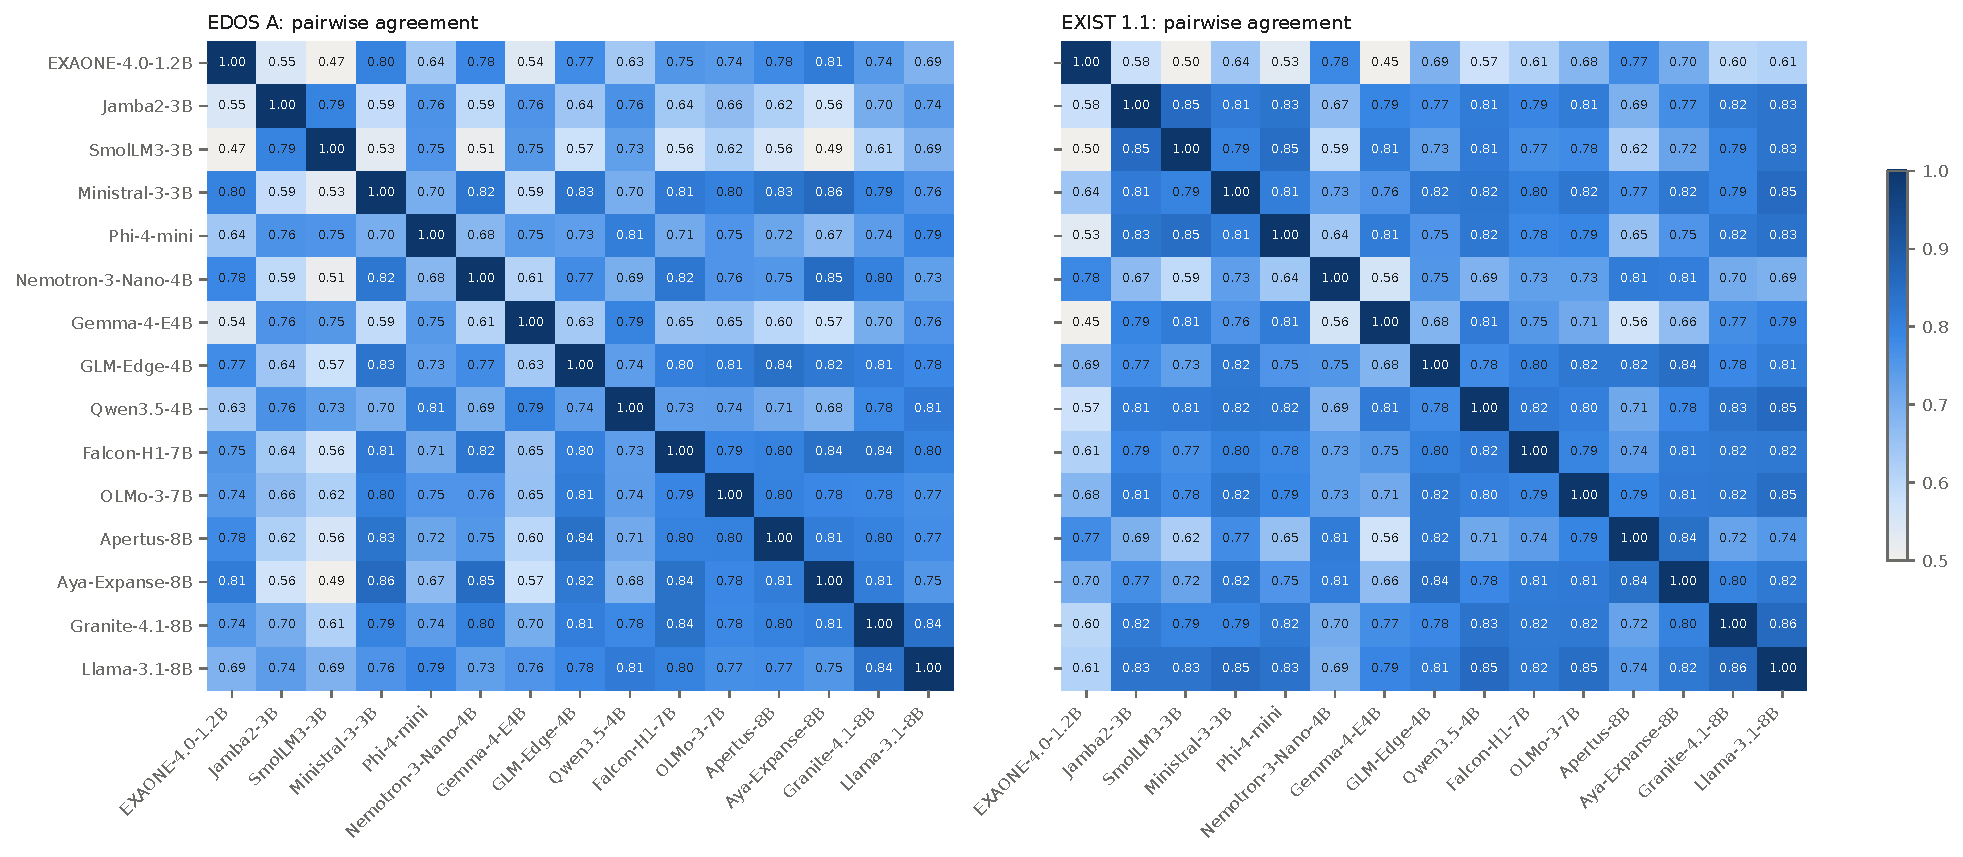
\includegraphics[width=\textwidth]{pairwise_agreement.pdf}
\caption{Share of test posts on which two models give the same prediction (refusal counts as its own prediction).}
\label{fig:pair}
\end{figure}

\end{document}
